\newcommand{\tabheader}     % Tabellenkopf
{
	\begin{zebratabular}[l]{@{}p{0.3\linewidth}p{0.3\linewidth}p{0.3\linewidth}p{0.06\linewidth}@{}}
		\rowcolor{gray}
		Anforderung &
		Pflicht &
		Wunsch &
		Verantw. \\
	}
\section{Aufgabenstellung}
\label{sec:aufgabe}
Es soll ein Gerät entwickelt werden, das Bälle in einen Korb werfen kann. 
Dies soll autonom erfolgen. 
\begin{figure}[h!]
    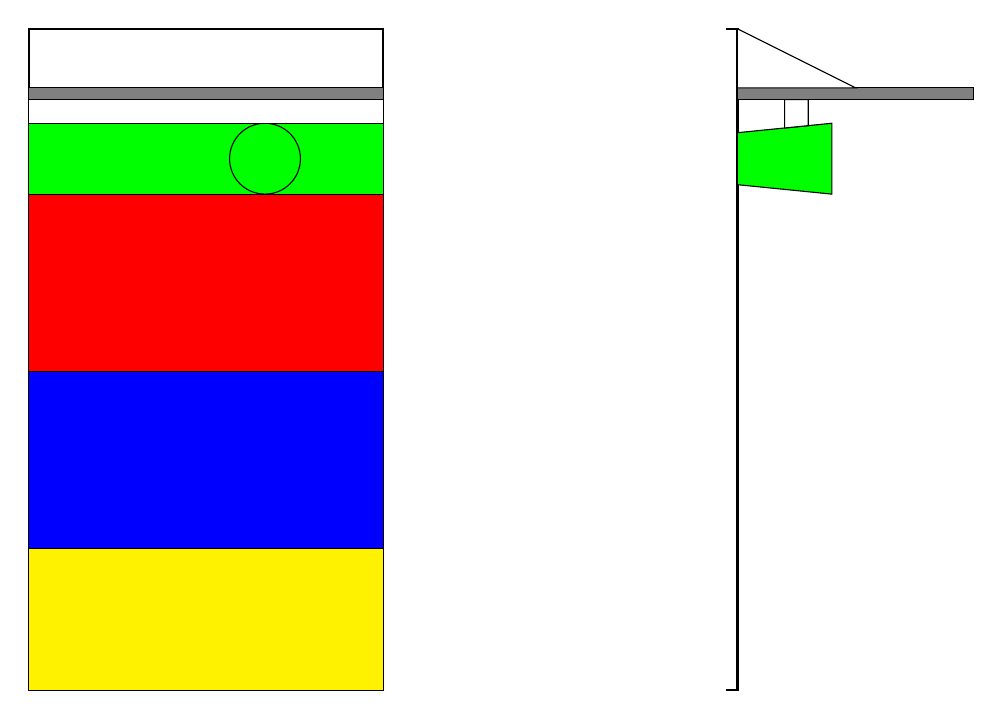
\begin{tikzpicture}[scale=0.03]
        % playfield frame
        \draw[thick] (0,0) rectangle (150,280);
        \draw[thick] (295,0) -- (300,0) -- (300,280) -- (295,280);
        % startfield
        \draw[fill=yellow] (0,0) rectangle (150,60);
        % move field
        \draw[fill=blue] (0,60) rectangle (150,135);
        % border line
        \draw[thick] (0,135) -- (150,135);
        % void field
        \draw[fill=red] (0,135) rectangle (150,210);
        % basket field
        \draw[fill=green] (0,210) rectangle (150,240);
        % basket
        \draw[fill=green] (100,225) circle [radius=15];
        \draw[fill=green] (300,214) -- (340,210) -- (340,240) -- (300,236) -- (300,214);
        % gap filler
        \draw[fill=white] (0,240) rectangle (150,250);
        \draw[fill=white] (320,250) -- (320,238) -- (330,239) -- (330,250) -- (320,250);
        % wall
        \draw[fill=gray] (0,250) rectangle (150,255);
        \draw[fill=gray] (300,250) rectangle (400,255);
        \draw[fill=white] (300,255) -- (350,255) -- (300,280) -- (300,255);
    \end{tikzpicture}
    \caption{Spielfeld}
    \label{fig:playfield}
\end{figure}
In diesem Kapitel werden die vorgegebenen Anforderungen an das Projekt 
besprochen. Dazu gehören Anforderungen an das Gerät sowie Rahmenbedingungen. 
In der Spalte Pflicht ist jeweils die Mindestanforderung beschrieben und in 
der Spalte Wunsch ist die vom Projektteam als Idealfall bezeichnete Leistung 
beschrieben. 
\subsection{Gerät}
\tabheader
	Abmessungen & 
	$\leq$ 50 cm x 50 cm x 100 cm &
	&
	M \\
	Gewicht &
	&
	$\leq$ 2 kg &
	M, E \\
	Startbefehl &
	drahtlos &
	drahtlos von Handy &
	E, I \\
	Übermittlung Endsignal &
	An gleiches Gerät wie Startsignal &
	&
	E, I \\
	Aufhängevorrichtung &
	Kann von Federwaage gewogen werden &
	&
	M \\
	Design &
	&
	Optisch ansprechend &
	M \\
	Korbfindung &
	selbständig &
	&
	E, I \\
	Stromversorgung &
	&
	Interne Stromversorgung &
	E \\
	\end{zebratabular}
	
	\subsection{Randbedingungen}
	\tabheader
	Abmessungen Spielfeld &
	$\geq$ 148 cm x 58 cm &
	&
	Doz \\
	Freie Höhe über Spielfeld &
	$\geq$ 1.8 m &
	&
	Doz \\
	Freier Raum um Spielfeld &
	$\geq$ 0.5 m &
	&
	Doz \\
	Distanz Mittellinie bis Korb &
	75 cm $\ldots$ 1.9 m &
	&
	Doz \\
	Personensicherheit &
	muss jederzeit gewährleistet sein &
	&
	E, I, M \\
	Sicheres Beenden der Aufgabe &
	&
	ohne Beschädigung des Gerätes &
	I \\
	Not-Ausschalter &
	vorhanden &
	manuelle Steuerung &
	E, I \\
	Budget &
	$\leq$ 600 Fr. &
	&
	E, I, M \\
	Gewicht Tennisball &
	55 $\ldots$ 59 g &
	&
	Doz \\
	Durchmesser Tennisball &
	6.3 $\ldots$ 7.3 cm &
	&
	Doz \\
	Durchmesser Korb &
	30 cm &
	&
	Doz \\
	Höhe Korb &
	40 cm &
	&
	Doz \\
	Einrichtzeit &
	$\leq$ 5 min &
	$\leq$ 2 min &
	E, I, M \\
\end{zebratabular}

\subsection{Eigene Anforderungen}
Es werden noch spezifisch an Flug- beziehungsweise Bodenobjekte eigene 
Anforderungen gestellt. 

\subsubsection{Flugobjekt}
\tabheader
	Dauer zur Erfüllung der Aufgabe &
	$\leq$3 min &
	1 min &
	E, I, M \\
	Effizienz &
	5 Bälle im Korb &
	&
	E, I, M \\
	Abfluggewicht &
	$\leq$2 kg (ohne Bälle) &
	$\leq$1 kg (ohne Bälle) &
	E, M \\
	Funktional &
	Fokus auf Funktion &
	&
	E, I, M \\
	Design &
	Leichtbau &
	Ansprechendes Design &
	M \\
	Special-Effects &
	&
	Beim Abschlusssignal soll ein Special-Effect ausgelöst werden (Konfetti, Rauch, usw.) &
	E, I, M \\
\end{zebratabular}


\subsubsection{Bodenobjekt}
\tabheader
	Dauer zur Erfüllung der Aufgabe &
	$\leq$3 min &
	1 min &
	E, I, M \\
	Effizienz &
	min. 3 Bälle im Korb &
	5 Bälle im Korb &
	E, I, M \\
	Gewicht &
	$\leq$8 kg &
	$\leq$2 kg &
	E, M \\
	Design &
	Elegantes, spezielles Design &
	abheben von Konkurrenz &
	M \\
	Special-Effects &
	Das Gerät kann min 1 Special-Effects (Konfetti, Rauch, Sound, usw.) &
	Das Gerät kann min 3 Special-Effects (Konfetti, Rauch, Sound, usw.) &
	E, I, M \\
\end{zebratabular}		
